%%%%%%%%%%%%%%%%%%%%%%% file template.tex %%%%%%%%%%%%%%%%%%%%%%%%%
%
% This is a general template file for the LaTeX package SVJour3
% for Springer journals.          Springer Heidelberg 2010/09/16
%
% Copy it to a new file with a new name and use it as the basis
% for your article. Delete % signs as needed.
%
% This template includes a few options for different layouts and
% content for various journals. Please consult a previous issue of
% your journal as needed.
%
%%%%%%%%%%%%%%%%%%%%%%%%%%%%%%%%%%%%%%%%%%%%%%%%%%%%%%%%%%%%%%%%%%%
%
% First comes an example EPS file -- just ignore it and
% proceed on the \documentclass line
% your LaTeX will extract the file if required
\begin{filecontents*}{example.eps}
%!PS-Adobe-3.0 EPSF-3.0
%%BoundingBox: 19 19 221 221
%%CreationDate: Mon Sep 29 1997
%%Creator: programmed by hand (JK)
%%EndComments
gsave
newpath
  20 20 moveto
  20 220 lineto
  220 220 lineto
  220 20 lineto
closepath
2 setlinewidth
gsave
  .4 setgray fill
grestore
stroke
grestore
\end{filecontents*}
%
\RequirePackage{fix-cm}
%
\documentclass{svjour3}                     % onecolumn (standard format)
%\documentclass[smallcondensed]{svjour3}     % onecolumn (ditto)
%\documentclass[smallextended]{svjour3}       % onecolumn (second format)
%\documentclass[twocolumn]{svjour3}          % twocolumn
%
\smartqed  % flush right qed marks, e.g. at end of proof
%
\usepackage{graphicx}
\usepackage{grffile}
\usepackage{bbding}
\usepackage[numbers,sort&compress]{natbib}
\usepackage{tabularx}
\usepackage[toc,page]{appendix}
%
% \usepackage{mathptmx}      % use Times fonts if available on your TeX system
%
% insert here the call for the packages your document requires
%\usepackage{latexsym}
% etc.
%
% please place your own definitions here and don't use \def but
% \newcommand{}{}
%
% Insert the name of "your journal" with
% \journalname{myjournal}
%

\begin{document}

\title{H-1B Visa classification and machine learning model evaluation%\thanks{Grants or other notes
%about the article that should go on the front page should be
%placed here. General acknowledgments should be placed at the end of the article.}
}
%\subtitle{H-1B Visa classification}

%\titlerunning{Short form of title}        % if too long for running head

\author{Lingfeng Zhang        \and
        Biliang Wang %etc.
}

%\authorrunning{Short form of author list} % if too long for running head

\institute{L. Zhang \at
              \email{lzhan278@uottawa.ca}           %  \\
%             \emph{Present address:} of F. Author  %  if needed
           \and
           B. Wang \at
              \email{bwang135@uottawa.ca} 
}

\date{Received: date / Accepted: date}
% The correct dates will be entered by the editor


\maketitle

\begin{abstract}
Getting a H-1B visa is crucial for internationals who want to pursue a professional career in US. A small fraction of applicants are denied each year  and they do have a definite reason. This work utilizes supervised learning and unsupervised learning (outlier detection) to classify visa applications, thus find the features that have the most prominent impact on application result. We also compare different machine learning models in comprehensive aspects, such as classification performance, training/testing speed and memory consumption rate, understanding the strength and limitations of  each model. Based on experimental results, we then make final conclusions.
\keywords{ Machine learning \and Model evaluation\and Outlier detection \and Supervised learning \and Unsupervised learning}
% \PACS{PACS code1 \and PACS code2 \and more}
% \subclass{MSC code1 \and MSC code2 \and more}
\end{abstract}

\section{Introduction}
\label{intro}

In recent years, an increasing number of internationals expect to get a working permission in US for various reasons. Among more than half of a million applicants each year, thousands of people are denied by the U.S. Citizenship and Immigration Service (USCIS). Applicants have many hypothesis and assumptions but never a deterministic reason for their denial. This work presents to apply machine learning techniques, including supervised learning, feature selection and resample techniques, to classify visa case status. We also address this task using outlier detection, which is an unsupervised learning method. Empowered by scikit-learn package, we are eager to discover features that have prominent impact on application result.

Another focus of this study is, with a comprehensive comparison and analysis, discussing the strength and limitations of different types of machine learning algorithm. Choosing $F_2$ score as evaluation criterion, we apply Friedman test to determine whether average ranks of model as a whole shows significant difference in classification performance and Nemenyi/Bonferroni–Dunn test to illustrate the critical difference on a pairwise level, along with other measurements, such as training/testing speed, memory consumption rate.

Finally, we give the conclusion according to the experiment results. Based on the exploration, hopefully, most applicants can anticipate an accurate visa decision by using our model.

This work is organized as follows. The next section describes the raw dataset used in this work. Section 3 explains data engineering procedure, model construction and experimental evaluation. Finally, section 4 concludes and outlines future research work.

\section{Case study}
We retrieve the dataset from Kaggle\citep{Anbarasan}, which is the raw data of H-1B visa application in 2018. The dataset has 654360 rows and 52 columns, and it is extremely skewed, only 1.3\% instances are positive class, meaning that 1.3\% applicants in 2018 are denied by USCIS. Main attributes, descriptions and feature values can be summarized in the Appendix \ref{appendix: table}.

For the sake of quick and smooth demonstration, we stratified approximate 20000 instances from the raw dataset for further process and analysis. The raw dataset is only used in outlier detection.
\section{Experimental setup and Evaluation}
Prior constructing the models, some feature engineering techniques are conducted on the dataset, in order to execute algorithms integrated in scikit-learn package. We then compare the models in terms of statistic difference, training/testing speed and memory consumption rate. The performance of outlier detection model is explained in the last part of this section.
\subsection{Feature Engineering}
Before feeding the data to machine learning algorithms, we apply several feature engineering methods to the dataset, including feature transformation, feature selection and resampling, creating nine new different datasets in this process.
\subsubsection{Feature transformation}
There are mainly three steps of feature transformation, deleting correlated columns, generating new columns and handling numerical and categorical data.
\paragraph{Deleting correlated columns} 
The raw dataset contains several correlated columns, such as employer state and worksite state, more than 90\% of rows have same data in these two columns. Hence, we delete one of the correlated columns to reduce information redundancy, which will reduce the effect of the curse of dimensionality simultaneously. Such columns are not displayed in Appendix \ref{appendix: table}.
\paragraph{Generating new columns} 
Additionally, we create some new features based on the original ones, which can better describe the visa application than before. 

Combine CASE\_SUBMITTED and DECISION\_DATA to create a new column called PROCESS\_TIME, which tells the duration of case processing in days.

Create column EMP\_PERIOD by subtracting column EMPLOYMENT\_END\_DATE and EMPLOYMENT\_STATE\_DATE, and we now have the length of working contract.

Despite all numbers, PREVAILING\_WAGE actually has different unit because some company pay employees monthly, while others on a weekly basis. We then add ANNUAL\_SALARY by multiplying  PREVAILING\_WAGE and PW\_UNIT\_OF\_PAY.

In common sense, these kinds of feature transformation can reduce the feature redundancy to ensure algorithms run faster and reduce the effect of curse of dimensionality. 
\paragraph{Handling numerical and categorical data} 
After the first phase of data processing, there are 11 numerical features and 10 categorical features in the dataset.

Numerical features are transformed in a num\_pipeline to fill the missing value with median value of each column, and then normalized with standard scaler. Categorical features, on the other hand, are fitted in a cat\_pipeline to fill the void with mode of individual column and are transferred into numerical values using one-hot encoder.  Some machine learning algorithms can only read numerical values, so it is essential to encoding categorical features into numerical values. Note that the amount of features is expanded after one-hot encoding.

The original dataset now is expanded to 20327 instances and 122 features which will be referred as OR for further experiments.
\subsubsection{Feature selection}
Feature selection is an ideal way of tackling the so called “curse of dimensionality” without significantly reducing the accuracy of model prediction.

We propose three ways of attributes reduction, Boruta\citep{Kursa}, L1-based\citep{Richard} and tree-based feature selection. The first one is implemented by scikit-learn-contrib, and the last two methods are integrated in standard scikit-learn package.

The number of attributes in original dataset is now reduced to 5, 9 and 16 after applying Boruta, L1-based and tree-based selection, respectively, which are shown in Table \ref{tab:feature selection}.

\begin{table}[h]
% table caption is above the table
\caption{Attributes selected by different methods}
\label{tab:feature selection}       % Give a unique label
% For LaTeX tables use
\begin{tabular}{cccc}
\hline\noalign{\smallskip}
Attribute  & Boruta & L1-based & Tree-based\\
\noalign{\smallskip}\hline\noalign{\smallskip}
PROCESS\_TIME & \Checkmark & \Checkmark & \Checkmark \\
ANNUAL\_SALARY & \Checkmark & \Checkmark & \Checkmark\\
SOC\_CODE\_15 & \Checkmark & \Checkmark &\\
H1B\_DEPENDENT\_N & \Checkmark & & \\
H1B\_DEPENDENT\_Y & \Checkmark & \Checkmark &\\
AGENT\_REPRESENTING\_EMPLOYER\_Y & & \Checkmark & \Checkmark\\
AGENT\_REPRESENTING\_EMPLOYER\_N & &  & \Checkmark\\
NAICS\_CODE\_54 & & \Checkmark & \Checkmark\\
FULL\_TIME\_POSITION\_Y & & \Checkmark &\\
WILLFUL\_VIOLATOR\_N & & \Checkmark & \\
SUPPORT\_H1B\_Y & & \Checkmark &\\
TOTAL\_WORKERS & & &  \Checkmark\\
NEW\_EMPLOYMENT & & &  \Checkmark\\
CONTINUED\_EMPLOYMENT & & &  \Checkmark\\
CHANGE\_PREV\_EMPLOYMENT & & &  \Checkmark\\
CHANGE\_EMPLOYER & & &  \Checkmark\\
AMENDED\_PETITION & & &  \Checkmark\\
EMP\_PERIOD & & &  \Checkmark\\
PW\_WAGE\_LEVEL\_LEVEL I & & &  \Checkmark\\
PW\_WAGE\_LEVEL\_LEVEL II & & &  \Checkmark\\
PW\_WAGE\_LEVEL\_LEVEL III & & &  \Checkmark\\
WORKSITE\_STATE\_CA & & &  \Checkmark\\
WORKSITE\_STATE\_NY & & &  \Checkmark\\
\noalign{\smallskip}\hline
\end{tabular}
\end{table}

Four of five attributes selected by Boruta are also picked by L1-based, while four of nine features in L1-based are chosen by tree-based. PROCESS\_TIME and ANNUAL\_SALARY are only two features that are selected by all three methods.
\subsubsection{Resampling}
Since the dataset is highly skewed, three types of resampling techniques are applied. Oversampling the minority class by random oversampling (ROS), Under-sampling the majority class with repeated edited nearest neighbors\citep{Wilson} (RENN) and Balanced sampling, which performs oversampling with Synthetic Minority Over-sampling Technique and cleaning using edited nearest neighbors\citep{Batista} (SMOTE-ENN). All the resampling algorithms are implemented by \citep{Guillaume}. Average class ratio and total instances of positive and negative before and after applying resampling are shown in the Table \ref{tab:resampling}.

\begin{table}[h]
% table caption is above the table
\caption{Class ratio and instance after resampling}
\label{tab:resampling}       % Give a unique label
% For LaTeX tables use
\begin{tabular}{ccccc}
\hline\noalign{\smallskip}
 & Original & ROS & RENN & SMOTE-ENN \\
\noalign{\smallskip}\hline\noalign{\smallskip}
Ratio & 0.0134 & 1.0000 & 0.0138 & 0.9905 \\
Total instance & 20327 & 40116 & 19815 & 33994 \\
\noalign{\smallskip}\hline
\end{tabular}
\end{table}

Compared with the original dataset, ROS and SMOTE-ENN inflate the dataset by increasing the positive class, whereas RENN only decreases a small number of negative class.
\subsection{Model evaluation}
\subsubsection{Defining datasets and models}
Ten datasets are produced during the feature engineering procedures. Details are illustrated in the following Table \ref{tab:dataset}.

\begin{table}[h]
% table caption is above the table
\caption{Dataset description}
\label{tab:dataset}       % Give a unique label
% For LaTeX tables use
\begin{tabular}{cccc}
\hline\noalign{\smallskip}
Dataset & Total instance & cls & Description \\
\noalign{\smallskip}\hline\noalign{\smallskip}
Original (OR) & 20327 & 0.0134 & No resampled and feature selection \\
Ros\_Boruta (RB) & 40116 & 1 & ROS resampled and Boruta selection\\
Ros\_L1 (RL) & 40116 & 1 & ROS resampled and L1-based selection\\
Ros\_Tr (RT) & 40116 & 1 & ROS resampled and Tree-based selection\\
Renn\_Boruta (EB) & 19753 & 0.0138 & RENN resampled and Boruta selection\\
Renn\_L1 (EL) & 19817 & 0.0138 & RENN resampled and L1-based selection\\
Renn\_Tr (ET) & 19875 & 0.0137 & RENN resampled and Tree-based selection\\
Smote\_Boruta (SB) & 31643 & 0.966 & SMOTE-ENN resampled and Boruta selection\\
Smote\_L1 (SL) & 32207 & 1.0045 & SMOTE-ENN resampled and L1-based selection\\
Smote\_Tr (ST) & 38132 & 1.0012 & SMOTE-ENN resampled and Tree-based selection\\
\noalign{\smallskip}\hline
\end{tabular}
\end{table}

This work presents six types of models, tree-based, linear, distance-based, probabilistic, rule-based and ensemble. For ensemble models, bagging, boosting and hybrid models have been trained, respectively. Basic theories of these models are illustrated by \citep{Peter}. This generates eight models, which are shown in the Table \ref{tab:model}.

\begin{table}[h]
% table caption is above the table
\caption{Model description}
\label{tab:model}       % Give a unique label
% For LaTeX tables use
\begin{tabular}{cc}
\hline\noalign{\smallskip}
Model & Description \\
\noalign{\smallskip}\hline\noalign{\smallskip}
DecisionTreeClassifier (DT) & Decision Tree algorithm\citep{Breiman} implemented by scikit-learn\\
LinearSVC (LE) & Support vector machine algorithm\citep{Yuan} implemented by scikit-learn\\
KNeighborsClassifier (KNN) & K-Nearest Neighbors algorithm\citep{Coomans} implemented by scikit-learn\\
GaussianNB (GNB) & Naive Bayes algorithm\citep{McCallum} implemented by scikit-learn\\
SkopeRules (SR) & Skope-rules algorithm implemented by scikit-learn-contrib\\
RandomForestClassifier (RF) & Random Forest algorithm\citep{Kam} implemented by scikit-learn\\
AdaBoostClassifier (AD) & Boosting algorithm\citep{Schapire} implemented by scikit-learn\\
VotingClassifier (VT) & Hybrid algorithm implemented by scikit-learn\\
\noalign{\smallskip}\hline
\end{tabular}
\end{table}

For LinearSVC model, we use kernel trick to change the hyperplane from linear to non-linear, which achieves the better result probably because the decision boundary of H1B visa classification task is non-linear. We use RBF kernel, which is a default kernel in LinearSVC probably because RBF kernel can work well for most of datasets.  SVM is tricky to tune if default kernel can not work well because several kernel tricks should be tested. If RBF kernel do not work in some cases, according to some articles, using polynomial kernel is also a good choice. The default maximum iteration is not enough for our dataset, which can not converge well, so we tune the hyper-parameter of maximum iteration from 2,000 to 20,000. In addition, The learning curve of LinearSVC is shown in Figure \ref{fig:learning_curve} . We can see the curve can fit well. 

\begin{figure}[h]
% Use the relevant command to insert your figure file.
% For example, with the graphicx package use
  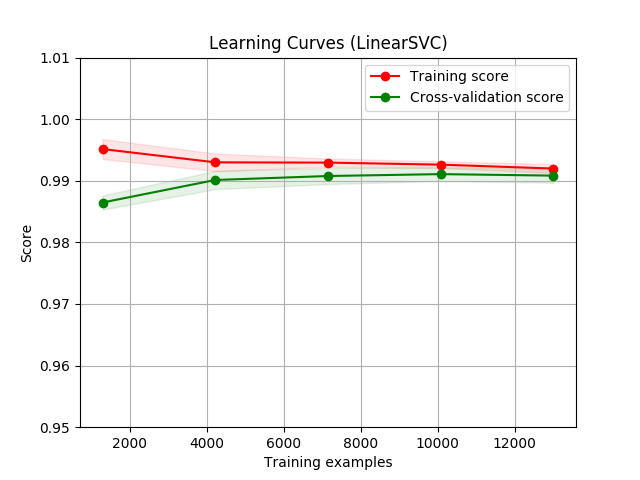
\includegraphics[width=0.75\textwidth]{linearsvc_learning_curve.png}
% figure caption is below the figure
\caption{Learning curve of LinearSVC}
\label{fig:learning_curve}       % Give a unique label
\end{figure}

For K nearest neighbour classifier, we use weighted distance, meaning closer the distance between two instances is, more weights the distance is given. Weighted KNN performs well in this case.

There is no good rule-based model in scikit-learn package. Dummy classifier a very simple rule-based model, only including one rule, like decision trump. So, this simple classifier can not work well for this large datasets with many features. Orange is another package, and it needs Anaconda environment to run the CN2 rule-based classifier. The shortcoming of Orange is that it costs too much time to run the model, meaning it is extremely slow to get the result. For our large dataset, using Orange to train the model is not a good idea. So we choose skope-rule as rule-based model, it is a higher level API based on scikit-learn API, which is convenient to be applied in our experiments.

\subsubsection{Evaluation criteria}
After all the models have been trained against ten datasets, we need to find a measurement to evaluate the models. For this binary classification problem, we care more about the positive class, the ones that are denied by the USCIS, over the negative class, the ones that are approved. Since the accuracy could not present whether a model is good or not in imbalanced dataset, precision and recall should be considered.

F-measure\citep{Nancy}, also $F_1$ score is a potential indicator, combing precision and recall, both of which are insensitive about true negatives. The definition of $F_1$ score is,
\begin{equation}
F_1 = 2 \cdot \frac{precision \cdot recall}{precision + recall}
\end{equation}
However, in this case, recall should be of more emphasis than precision, as we want the false negative to be as small as possible, which means the number of cases such that classified by the model as approved are in fact denied should be minimized.

Based on the idea above, we thus choose $F_2$ score\citep{Van}, which weights recall higher than precision. The definition of $F_2$ score is:
\begin{equation}
F_2 = (1 + \beta ^2) \cdot \frac{precision \cdot recall}{(\beta ^2 \cdot precision) + recall}
\end{equation}
Where $\beta = 2$. The $F_2$ score of models trained against each dataset can be found in the Table \ref{tab: F2 score}.

\begin{table}[h]
% table caption is above the table
\caption{$F_2$ score of models}
\label{tab: F2 score}       % Give a unique label
% For LaTeX tables use
\begin{tabular}{ccccccccc}
\hline\noalign{\smallskip}
 & DT & LE & KNN &  GNB & SR & RF & AD & VT \\
\noalign{\smallskip}\hline\noalign{\smallskip}
OR & 0.7770 & 0.6582 & 0.6809 & 0.2377 & 0.8204 & 0.7599 & 0.7842 & 0.6986 \\
RB & 0.9759 & 0.8529 & 0.9690 & 0.7014 & 0.8790 & 0.9762 & 0.8964 & 0.9781\\
RL & 0.9814 & 0.8273 & 0.9710 & 0.7865 & 0.8496 & 0.9799 & 0.8854 & 0.9820\\
RT & 0.9838 & 0.8090 & 0.9810 & 0.6318 & 0.8495 & 0.9913 & 0.9004 & 0.9925\\
EB & 0.8442 & 0.7033 & 0.8485 & 0.8060 & 0.8184 & 0.8421 & 0.8290 & 0.8499\\
EL & 0.7935 & 0.7207 & 0.8105 & 0.5668 & 0.8179 & 0.8192 & 0.8279 & 0.7999\\
ET & 0.8268 & 0.6703 & 0.7970 & 0.4468 & 0.8223 & 0.8370 & 0.8310 & 0.8369\\
SB & 0.9864 & 0.9222 & 0.9895 & 0.8021 & 0.9482 & 0.9891 & 0.9734 & 0.9887\\
SL & 0.9786 & 0.8812 & 0.9818 & 0.8609 & 0.9055 & 0.9859 & 0.9618 & 0.9790\\
ST & 0.9820 & 0.8312 & 0.9826 & 0.7185 & 0.8746 & 0.9925 & 0.9690 & 0.9823\\
\noalign{\smallskip}\hline\noalign{\smallskip}
avg & 0.8795 & 0.7447 & 0.8318 & 0.4781 & 0.8475 & 0.8762 & 0.8766 & 0.8405\\
stdev & 0.1450 & 0.1224 & 0.2133 & 0.3400 & 0.0383 & 0.1645 & 0.1306 & 0.2005\\
\noalign{\smallskip}\hline
\end{tabular}
\end{table}

This preliminary compare shows, on average, Decision Tree has the highest $F_2$ score, closely followed by Random Forest, Adaboost. Naive Bayes has the lowest $F_2$ score, average below 50\% for binary classification, which means Naive Bayes classifier is a weak learner. This is possibly because features are not mutually independent and the Naive Bayes classifier applies Bayes’ theorem with strong independent assumptions between the features. 

The comparison also emphasizes that, given a model, $F_2$ score generated from original dataset is lower than other dataset, which means feature reduction and  resampling may, at some degree, increase the classification performance. Additionally, models trained against under-sampling datasets perform less satisfied than oversampling and balanced sampling ones. This is probably because of information loss in the cleaning process. Another reason is that under sampling rate in this case is low, which means the resampling method do not under sample the majority class too much. So the result of under sampling dataset do not improve significantly compared with the result of without sampling dataset.

Further test will be conducted to focus on whether average ranks of $F_2$ score as a whole displays significant differences.

\subsubsection{Friedman test}
Friedman test\citep{Friedman} is designed for testing $k$ algorithms against $n$ datasets. Table \ref{tab: avg ranks} shows ranks of $F_2$ score.

\begin{table}[h]
% table caption is above the table
\caption{Ranks of $F_2$ score}
\label{tab: avg ranks}       % Give a unique label
% For LaTeX tables use
\begin{tabular}{ccccccccc}
\hline\noalign{\smallskip}
 & DT & LE & KNN &  GNB & SR & RF & AD & VT \\
\noalign{\smallskip}\hline\noalign{\smallskip}
OR & 3 & 7 & 6 & 8 & 1 & 4 & 2 & 5 \\
RB & 3 & 7 & 4 & 8 & 6 & 2 & 5 & 1\\
RL & 2 & 7 & 4 & 8 & 6 & 3 & 5 & 1\\
RT & 3 & 7 & 4 & 8 & 6 & 2 & 5 & 1\\
EB & 3 & 8 & 2 & 7 & 6 & 4 & 5 & 1\\
EL & 6 & 7 & 4 & 8 & 3 & 2 & 1 & 5\\
ET & 4 & 7 & 6 & 8 & 5 & 1 & 3 & 2\\
SB & 4 & 7 & 1 & 8 & 6 & 2 & 5 & 3\\
SL & 4 & 7 & 2 & 8 & 6 & 1 & 5 & 3\\
ST & 4 & 7 & 3 & 8 & 6 & 1 & 5 & 2\\
\noalign{\smallskip}\hline\noalign{\smallskip}
avg & 3.5 & 7.0 & 4.5& 8.0 & 3.5 & 2.5 & 3.5 & 3.5\\
\noalign{\smallskip}\hline
\end{tabular}
\end{table}

Based on the Friedman test, $\overline{R} = \frac{k+1}{2} = 4.5$, $n\displaystyle\sum_{j}^{} (R_j - \overline{R})^2 = 265.0$  and $\frac{1}{n(k - 1)}\displaystyle\sum_{ij}^{} (R_{ij} - \overline{R})^2 = 6$, so the Friedman statistic is $44.2$. The critical value for $k = 8$ and $n = 10$ at the $\alpha = 0.05$ level is $14.1$, so we reject the null hypothesis that all algorithms perform equally, which means that the average ranks as a whole, at $\alpha = 0.05$  level, shows a significant difference.

\subsubsection{Nemenyi test}
Further analysis is carried out on a pairwise level. The critical difference in  Nemenyi test\citep{Nemenyi} is as follows:
\begin{equation}
\label{eqn:cd}
CD = q_\alpha \sqrt[]{\frac{k(k + 1)}{6n}}
\end{equation}
where $q_\alpha$ depends on the significance level $\alpha$ as well as $k$: for $\alpha = 0.05$ and $k = 8$ it is $3.03$, leading to a critical difference of $3.320$. There is significant difference between eight algorithms.

% For one-column wide figures use
\begin{figure}[h]
% Use the relevant command to insert your figure file.
% For example, with the graphicx package use
  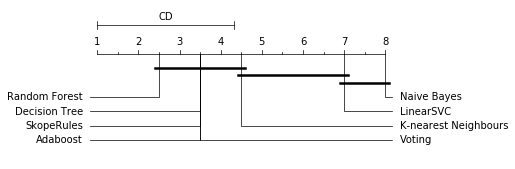
\includegraphics[width=0.75\textwidth]{Nemenyi diagram.png}
% figure caption is below the figure
\caption{Critical difference diagram for the pairwise Nemenyi test}
\label{fig:Nemenyi test}       % Give a unique label
\end{figure}

Figure \ref{fig:Nemenyi test} shows that RF, DT, SR, AD and VT are significantly better than LE and GNB. The reason why linear support vector classier performs not good is probably the decision boundary in this binary classification dataset is not clear and difficult to learn.

\subsubsection{Bonferroni–Dunn test}
Similar with Nemenyi test, Bonferroni–Dunn test can be used when we apply pairwise test only over a control algorithm. The calculation of critical difference is as same as Equation \ref{eqn:cd}, though $q_\alpha$ becomes $2.450$ in this case, hence the critical difference of Bonferroni–Dunn test is $2.947$. 

\begin{figure}[h]
% Use the relevant command to insert your figure file.
% For example, with the graphicx package use
  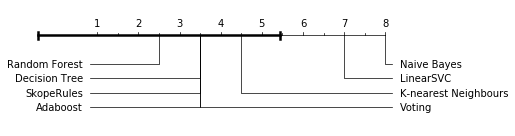
\includegraphics[width=0.75\textwidth]
  {BD diagram.png}
% figure caption is below the figure
\caption{Critical difference diagram for the pairwise Bonferroni–Dunn test}
\label{fig:BD test}       % Give a unique label
\end{figure}
Figure \ref{fig:BD test} shows Bonferroni–Dunn test using RF as control algorithm, we can generate similar conclusion as in Nemenyi test.

\subsection{Comparing algorithm computational resource}
Beyond the statistic tests, we also conduct comparison of computational resource in terms of training/testing speed and memory consumption rate of machine learning models. Related experiments are based on Google Colab default CPU environment and the computer with GPU in the laboratory.

\subsubsection{Training and testing speed}
We focus on speed of training a model because it is a particularly important measurement of distinguishing models when, in practice, the volume of data is seems to be enormous. For quantification purpose, we used instance per second as measuring metrics.

In order to measure these speed, a controlled experiment should be conducted. We feed the algorithms with a fixed dataset, RT, the one with the most features and instances.

\begin{figure*}
% Use the relevant command to insert your figure file.
% For example, with the graphicx package use
  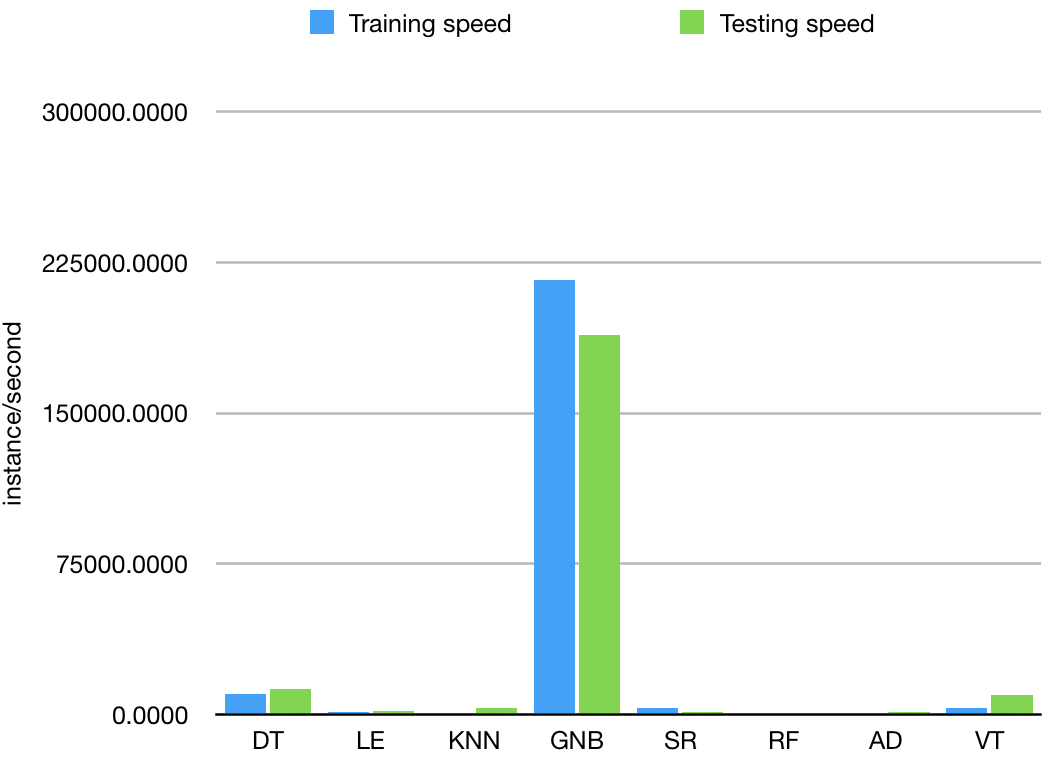
\includegraphics[width=0.75\textwidth]
  {training speed all.png}
% figure caption is below the figure
\caption{Training and testing speed of models}
\label{fig: Training speed all}       % Give a unique label
\end{figure*}

Figure \ref{fig: Training speed all} illustrates that, despite poor classification performance, Naive Bayes algorithm has unmatched advantage over other seven algorithms in terms of training and testing speed. It is fair to say that Naive Bayes is the “fastest” algorithm among the eight algorithms mentioned in this work. This is because Naive Bayes classifier is simply calculate different kinds of probability of the dataset. 

\begin{figure*}
% Use the relevant command to insert your figure file.
% For example, with the graphicx package use
  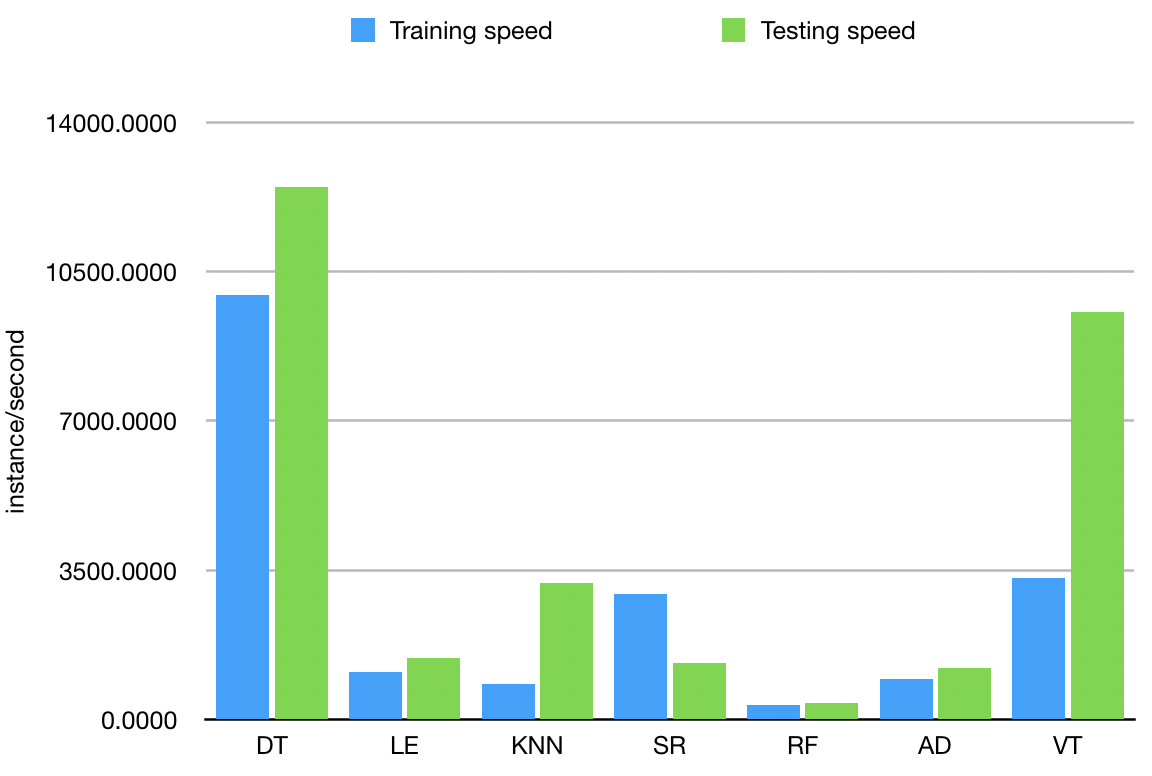
\includegraphics[width=0.75\textwidth]
  {training speed seven.png}
% figure caption is below the figure
\caption{Training and testing speed of models except Naive Bayes}
\label{fig: Training speed seven}       % Give a unique label
\end{figure*}

Figure \ref{fig: Training speed seven} provides a closer view of algorithms excluding Naive Bayes. Having the best classification performance, Random forest algorithm actually requires the “longest” time to build a model and test unseen data. Though Decision Tree, SkopeRules, Adaboost and Voting have the same average ranks in Friedman test, their speed performance has huge difference. Decision Tree is significantly faster than other three algorithms. An interesting discovery is that the testing speed of Voting and K-Nearest Neighbors algorithm are almost three times of their training speed.

Further analysis focuses on whether the size of dataset has impact on training and testing speed. We choose RF, the “slowest” algorithm to illustrate this experiment.

\begin{figure*}
% Use the relevant command to insert your figure file.
% For example, with the graphicx package use
  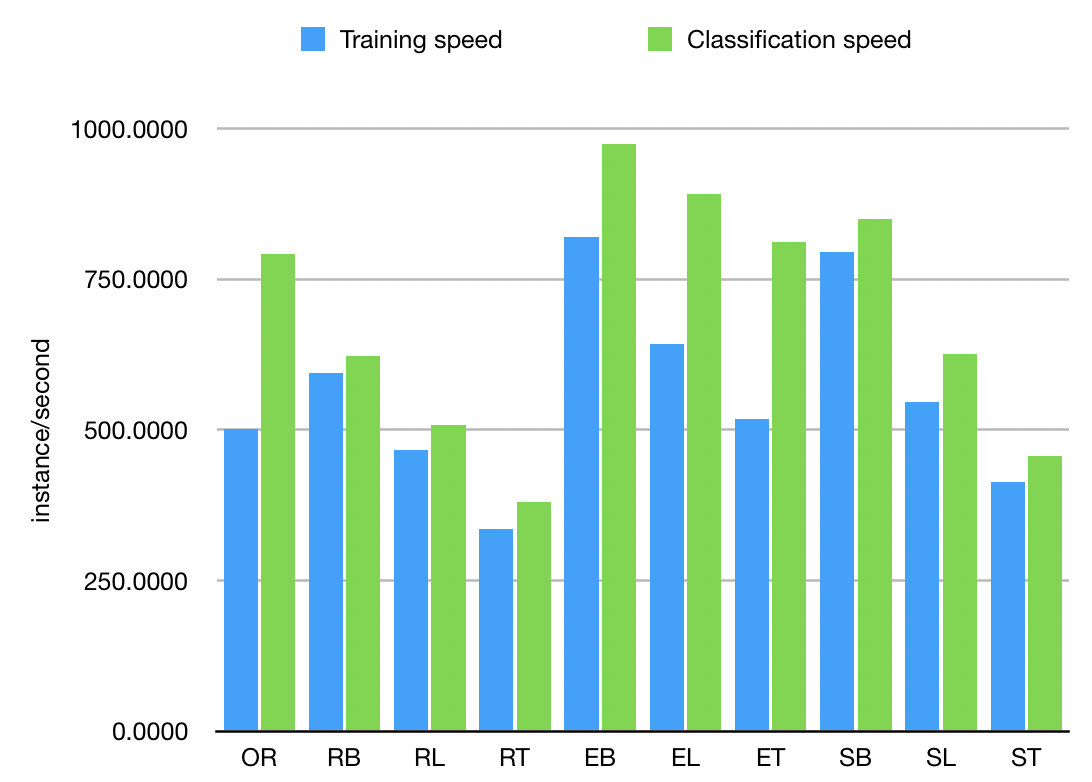
\includegraphics[width=0.75\textwidth]
  {training speed rf.png}
% figure caption is below the figure
\caption{Training and testing speed of Random Forest models on ten datasets}
\label{fig: Training speed rf}       % Give a unique label
\end{figure*}

Figure \ref{fig: Training speed rf} shows training and testing speed of RF on ten datasets. Given a resampling technique, say Boruta, speed performance on under-sampled and balanced sampled datasets is better than oversampled datasets, as the former two have fewer instances than the latter. In addition, given a feature selection method, say ENN, dataset with fewer features get faster training and testing speed. Generally speaking, the smaller the size of dataset is, the better speed performance ML algorithm has.

\subsubsection{Accelerating Machine Learning Algorithms by using Nvidia GPU}
Nvidia GPU is massively used in deep learning algorithms to accelerate the training speed significantly. Whether this powerful hardware can be applied in conventional machine learning algorithms? The answer is yes. The cuML is a RAPIDS Machine Learning Library and “cu” in the word “cuML” means NVIDIA CUDA. This library works similar as scikit-learn, including several supervised and unsupervised machine learning algorithms but not all. This is because some algorithms do not need a large amount of parallel computations, such as Naive Bayes, and this library is still developing.

In this experiment, we use Random Forest classifier (slowest classifier in this case) in both scikit-learn and cuML libraries to train and test bigger dataset (around 574,522 and 139 features after one hot encoder). In this way, we can see the significant difference between CPU computing speed and GPU computing speed. In addition, we do not use 10-fold cross validation in this comparison experiment because we only need to see training and testing speed separately. The result is shown in Table \ref{tab:gpu}.

\begin{table}[h]
% table caption is above the table
\caption{Traing and tesing time using CPU and GPU}
\label{tab:gpu}       % Give a unique label
% For LaTeX tables use
\begin{tabular}{clclc}
\hline\noalign{\smallskip}
 & Traing & Testing  \\
\noalign{\smallskip}\hline\noalign{\smallskip}
CPU & 295.43s & 0.57s \\
GPU & 47.21s & 1.07s \\
\noalign{\smallskip}\hline
\end{tabular}
\end{table}

For this dataset, GPU-based Random Forest can compete six times faster than the CPU equivalent in training. As for testing, using GPU is slightly slow. This is probably because the testing time contains the time of moving testing data from CPU to GPU. However, it still fast in testing section.

\subsubsection{Memory consumption rate}
Memory consumption rate is another key factor when comparing machine learning algorithms. Generally, it describes the memory requirement for building a model. In order to quantify the performance, we use Byte per instance as measuring metrics. Again, we use RT dataset as the input of this experiment.

\begin{figure*}
% Use the relevant command to insert your figure file.
% For example, with the graphicx package use
  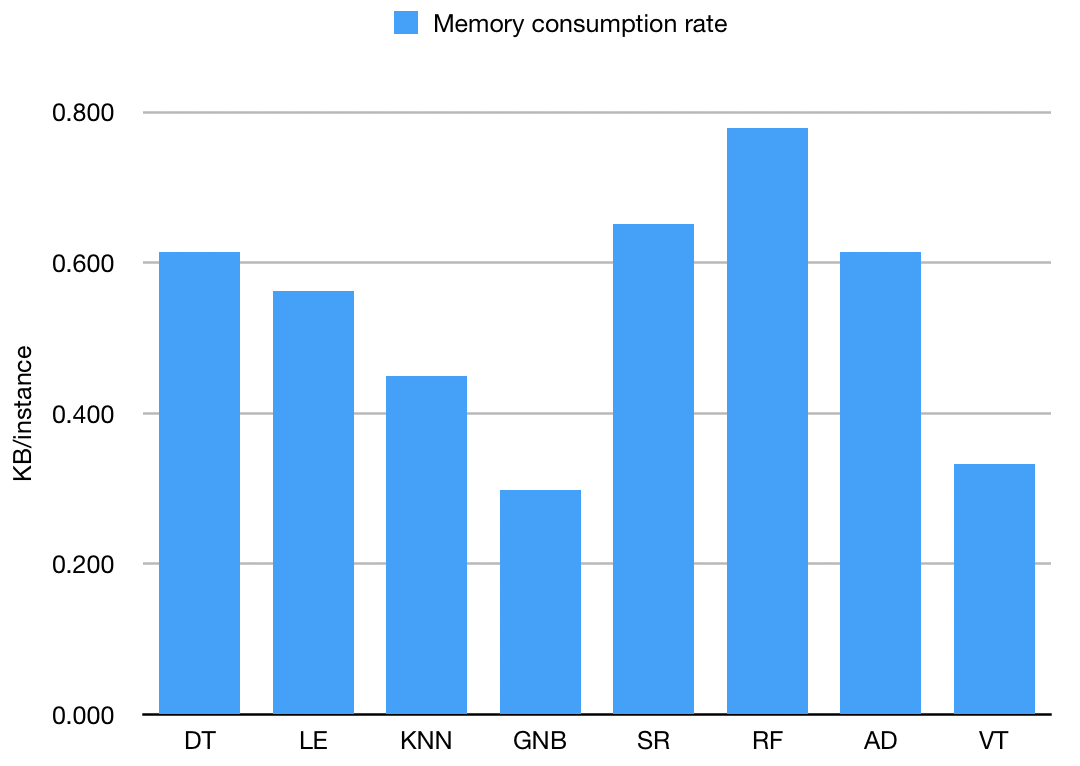
\includegraphics[width=0.75\textwidth]
  {memory.png}
% figure caption is below the figure
\caption{Memory consumption rate of models}
\label{fig: memory consumption rate}       % Give a unique label
\end{figure*}

Figure \ref{fig: memory consumption rate} illustrates that GNB algorithm needs the least memory to build a model, closely followed by VT. Similar as training/testing speed, RF algorithm  requires the most memory block than other seven algorithms.

The reason why GNB classifier needs less memory is probably because Naive Bayes classifier only need save two prior probabilities of two classes and several posterior probabilities with the condition of different classes in this case. As for decision tree, this model needs more memory to store various branches, which is a memory-intensive classifier. Moreover, Random forest has many trees, so it cost more memory. In addition, skope-rule classifier is a rule-based classifier but it is a modification of random forest, it passes a bagging estimator which uses several decision trees and regression trees and generate high performing and heterogeneous rules. So, skope-rule classifier is also a memory-intensive classifier. 

As for Linear Support Vector Classifier, how much memory it uses is depends on how large the kernel matrix is and how many support vectors it has, because if the kernel matrix is not stored, it will be recomputed repeatedly, making training much slower. Besides, SVM takes a linear combination with all support vectors, so it stores all support vectors.

For these memory-intensive models, it is  problematical to deploy these models in low-memory devices, such as smart phones and other small gadgets. 
\subsection{Outlier Detection}
In most cases, if the dataset is extremely skewed, outlier detection may be a good method to detect outliers (minority), but not always. Outlier detection is an unsupervised machine learning algorithm. We use training data without label to train the outlier detection model and use testing data with label to evaluate the model. So, recall (sensitivity) are also good metrics to evaluate the outlier detection model.

Using majority (inliers) with some minority (outliers) as training set let one class SVM learn the decision boundary relatively easy, compared with "clean" majority as training set. 

The result for some metrics is bad, where accuracy is around 0.5, and precision is about 0.02. This is possibly because the decision boundary in this dataset is unclear and difficult to learn and it has also been illustrated in the performance of linear support vector classifier. However, the recall is high, above 80$\%$. In this application, we care more about whether a failure case can be predicted as failure, and predicting a success case as failure is acceptable to some extents.

In the outlier detection, imbalanced dataset should not be sampled by using sampling methods. The performance of model is still not sufficient when it is feed the raw dataset which is containing 500,000 instances. We have tried other one class learning algorithms, like elliptic envelope and isolation forest in scikit-learn package. Still, the results are not convincing.

Novelty detection is the next step of evaluation, which wonderfully meets the definition of one class learning, only learning one class (majority). We only use majority without being polluted by minority to fit OneClassSVM, respectively. Yet the performance is not convincing, although recall slightly higher than that of the outlier detection model.

See Table \ref{tab:differ_outlier_detec}, we compare three one class learning models, OneClassSVM get the highest recall, significantly higher than other two one class learning model.

\begin{table}[h]
% table caption is above the table
\caption{Different Outlier Detection Models Recall}
\label{tab:differ_outlier_detec}       % Give a unique label
% For LaTeX tables use
\begin{tabular}{clclclc}
\hline\noalign{\smallskip}
 & OneClassSVM & EllipticEnvelope & IsolationForest  \\
\noalign{\smallskip}\hline\noalign{\smallskip}
Recall & 87.23$\%$ & 21.28$\%$ & 25.53$\%$ \\
\noalign{\smallskip}\hline
\end{tabular}
\end{table}


In addition, see Table \ref{tab:novelty}, we compare the different performance of training dataset including majority and minority, as well as training dataset including only majority. Only choosing majority as the training dataset  can slightly improve the performance of OneClassSVM in this case.

\begin{table}[h]
% table caption is above the table
\caption{Recall of outlier detection and novelty detection}
\label{tab:novelty}       % Give a unique label
% For LaTeX tables use
\begin{tabular}{clclc}
\hline\noalign{\smallskip}
 & majority with minority & "clean" majority  \\
\noalign{\smallskip}\hline\noalign{\smallskip}
Recall & 87.23$\%$ & 91.49$\%$ \\
\noalign{\smallskip}\hline
\end{tabular}
\end{table}

So, the conclusion about outlier detection model we can get is outlier detection can work, but not outperform than other classifiers with sampling methods.

The information we can get is that the decision boundary of this dataset is extremely unclear and hard to learn. Whether existing an outlier detection model which can detect outliers good enough should be done in the future work.

\subsection{Other metrics to evaluate imbalanced dataset}
\subsubsection{ROC curve and AUC area}

See Figure \ref{fig: roc_curve_sum} , when we use ROC curve to evaluate these models with imbalanced dataset, boosting achieves best and Naive Bayes is worst because AUC area of boosting is largest and that of Naive Bayes is smallest.

\begin{figure*}
% Use the relevant command to insert your figure file.
% For example, with the graphicx package use
  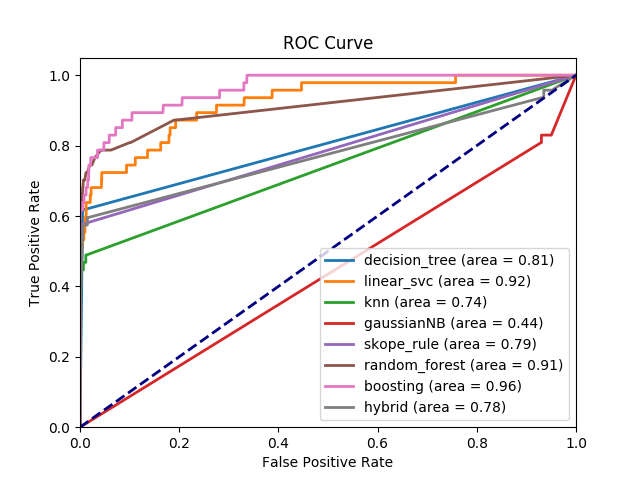
\includegraphics[width=0.75\textwidth]
  {roc_curve_sum.png}
% figure caption is below the figure
\caption{ROC curve with AUC area}
\label{fig: roc_curve_sum}       % Give a unique label
\end{figure*}

\subsubsection{Average recall}

For imbalanced dataset, although accuracy is not a good choice to evaluate the model, average accuracy is a relatively good metric.

\begin{equation}
average \ accuracy=\frac{1}{2}[\pi_{\textrm{positive}}+\pi_{\textrm{negative}}]
\end{equation}

where,

\begin{equation}
\pi_{\textrm{positive}}=TP/(TP+FN)
\end{equation}

\begin{equation}
\pi_{\textrm{negative}}=TN/(TN+FP)
\end{equation}

See Table \ref{tab:average_accuracy} or Figure \ref{fig: average_accuracy_png}, decision tree achieves best result and this is probably because decision tree is robust for class imbalance. Sometimes, decision tree is easy to conduce overfitting and random forest can tackle this issue. These ensemble classifier can achieve high average accuracy, too.

\begin{table}[h]
% table caption is above the table
\caption{average accuracy of different models}
\label{tab:average_accuracy}       % Give a unique label
% For LaTeX tables use
\begin{tabular}{clc}
\hline\noalign{\smallskip}
classifier & average accuracy  \\
decision tree & 0.81 \\
linear svc & 0.65 \\
knn & 0.68 \\
gaussianNB & 0.45 \\
skope rule & 0.79 \\
random forest & 0.80 \\
boosting & 0.80 \\
hybrid & 0.76 \\
\noalign{\smallskip}\hline
\end{tabular}
\end{table}

\begin{figure*}
% Use the relevant command to insert your figure file.
% For example, with the graphicx package use
  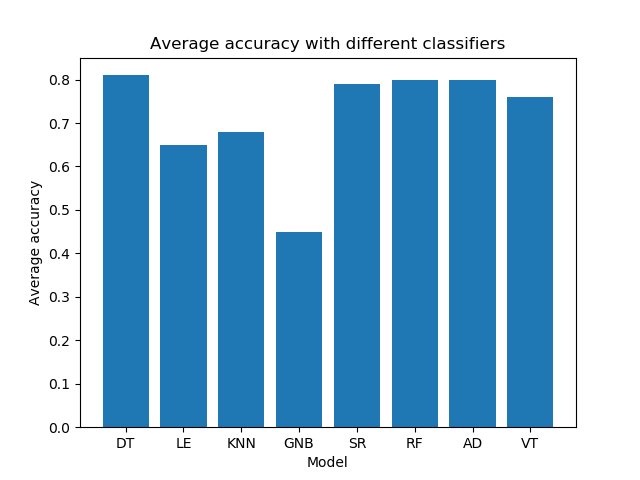
\includegraphics[width=0.75\textwidth]
  {average_accuracy.png}
% figure caption is below the figure
\caption{Average Accuracy Plot}
\label{fig: average_accuracy_png}       % Give a unique label
\end{figure*}

There are several metrics to evaluate the performance of classifiers based on a certain dataset. For imbalanced dataset, accuracy is not a good metric because majority dominates the result and recall, precision, average accuracy, roc curve, auc area and F-measure are good metrics. In the H-1B visa classification datasets, $F_2$ measure is the best metric we choose because recall should be given more emphasis than precision.

\section{Conclusion}
In this paper, we apply several statistical tests to select the model that is the most suitable for visa classification task. Besides, we conduct other experiments to compare models in different aspects, including training and testing speed and memory consumption rate.

We find that, using $F_2$ score as evaluation criterion, Random Forest, Decision Tree, SkopeRules, Adaboost and Voting are significantly better than Naive Bayes and LinearSVC in Friedman test, while in Nemenyi and Bonferroni–Dunn test, Random Forest, Decision Tree, SkopeRules, Adaboost, Voting and K-Nearest Neighbors do not display critical difference, although Random Forest is slightly better than them.

In the experiments of comparing training/testing speed and memory consumption rate, however, we find different result. Naive Bayes, which performs the worst in statistical tests, excels all other algorithms. In contrast, Random Forest is the “slowest” and most “greedy” algorithm.

Another finding is that feature selection and resampling techniques shows influence on training and testing speed. Generally speaking, the less number of instances and features the dataset has, the better speed performance ML algorithm possesses.

Last finding is that using GPU can accelerate the training speed in conventional machine learning models significantly. The dataset sometimes is extremely large in practical, it is time-consuming to train the model. If the model training part can be accelerated, it will save a considerable amount of time, which has a realistic significance.

To summarize, due to the no free lunch theorem, no one certain classifier and some certain methods can apply for any cases or datasets and achieve the best result. So, according to our experiments, using SMOTE-ENN balanced sampling and tree-based feature selection as dataset precessing and random forest classifier as training model can achieve the best result for H-1B visa classification task. In practical field, random forest training model can use cuML package or CUDA programming methods to accelerate the training speed with the power of Nvidia GPU. 

As this paper only exhibits preliminary investigations, we need some in-depth evaluations about why statistical discrepancies show in classification performance among models and whether there is a trade-off between accuracy and computational resources. We would also like to explore new methods of feature engineering, such that can improve the classification performance of a model. In addition, we would find a good outlier detection model to handle this imbalanced dataset even though common-used classifiers can perform well after resampling.




%\begin{acknowledgements}
%If you'd like to thank anyone, place your comments here
%and remove the percent signs.
%\end{acknowledgements}


% Authors must disclose all relationships or interests that 
% could have direct or potential influence or impart bias on 
% the work: 
%
% \section*{Conflict of interest}
%
% The authors declare that they have no conflict of interest.


% BibTeX users please use one of
%\bibliographystyle{spbasic}      % basic style, author-year citations
%\bibliographystyle{spmpsci}      % mathematics and physical sciences
%\bibliographystyle{spphys}       % APS-like style for physics
%\bibliography{reference.bib}   % name your BibTeX data base

% Non-BibTeX users please use
\begin{thebibliography}{}
%
% and use \bibitem to create references. Consult the Instructions
% for authors for reference list style.
%

\bibitem{Anbarasan}
A. Anbarasan: H1B Prediction, https://www.kaggle.com/abishekanbarasan1995/h1b-case-status-prediction.
\bibitem{Kursa}
% Format for Journal Reference
Kursa M., Rudnicki W., Feature Selection with the Boruta Package,  Journal of Statistical Software, Vol. 36, Issue 11, (2010)
\bibitem{Richard}
Richard G. Baraniuk, Compressive Sensing, IEEE Signal Processing Magazine, Vol. 24, (2007)
\bibitem{Wilson}
D. Wilson, Asymptotic, Properties of Nearest Neighbor Rules Using Edited Data, IEEE Transactions on Systems, Man, and Cybernetrics, vol. 2 (3), pp. 408-421, (1972)
\bibitem{Batista}
G. Batista, B. Bazzan, M. Monard, Balancing Training Data for Automated Annotation of Keywords: a Case Study, WOB, 10-18, (2003)
\bibitem{Guillaume}
Guillaume  Lema{{\^i}}tre and Fernando Nogueira and Christos K. Aridas, Imbalanced-learn: A Python Toolbox to Tackle the Curse of Imbalanced Datasets in Machine Learning, Journal of Machine Learning Research, Vol. 18, pp. 1-5, (2017)
\bibitem{Yuan}
Guo-Xun Yuan, Chia-Hua Ho, Chih-Jen Lin, Recent Advances of Large-Scale Linear Classification, Proc. IEEE. Vol. 100, No. 9, pp. 2584-2603, (2012)
\bibitem{Coomans}
D. Coomans, D.L. Massart, Alternative k-nearest neighbour rules in supervised pattern recognition : Part 1. k-Nearest neighbour classification by using alternative voting rules, Analytica Chimica Acta, Vol. 136, pp. 15–27,  (1982)
\bibitem{McCallum}
McCallum, Andre, Nigam, Kamal, A comparison of event models for Naive Bayes text classification, AAAI-98 workshop on learning for text categorization,  (1998)
\bibitem{Kam}
Ho, Tin Kam, Random Decision Forests, Proceedings of the 3rd International Conference on Document Analysis and Recognition, pp. 278–282, (1995)
\bibitem{Schapire}
Schapire, Robert E, The Strength of Weak Learnability, Machine Learning, Vol. 5, pp. 197–227, (1990) 
\bibitem{Nancy}
Nancy Chinchor, MUC-4 Evaluation Metrics, Proc. of the Fourth Message Understanding Conference, pp. 22–29, 1992.
% Format for books
\bibitem{Breiman}
Breiman, Leo, Friedman, J. H., Olshen, R. A., Stone, C. J., Classification and regression trees, Monterey, CA: Wadsworth \& Brooks/Cole Advanced Books \& Software, (1984)
\bibitem{Peter}
Peter Flach, Machine Learning: The art and science of algorithms that make sense of data, Cambridge University Press, (2012)
\bibitem{Van}
Van Rijsbergen, C. J., Information Retrieval (2nd ed.), Butterworth-Heinemann, (1979)
\bibitem{Friedman}
Friedman, Milton, A comparison of alternative tests of significance for the problem of m rankings, The Annals of Mathematical Statistics, Vol. 11, pp. 86–92, (1940)
\bibitem{Nemenyi}
Nemenyi, P.B., Distribution-free Multiple Comparisons, PhD thesis, Princeton University, (1963).
% etc
\end{thebibliography}

\begin{appendices}
\section{Dataset Description}
\label{appendix: table}

\begin{table}[h]
% table caption is above the table
%\caption*{Dataset description}
\label{tab:raw dataset}       % Give a unique label
% For LaTeX tables use
\begin{tabularx}{\textwidth}{|c|X|}
\hline\noalign{\smallskip}
Attribute & Description \\
\noalign{\smallskip}\hline\noalign{\smallskip}
CASE\_STATUS & Status associated with the last significant event or decision. Valid values include “Certified” and “Denied” \\\hline
CASE\_SUBMITTED & Date and time the application was submitted\\\hline
DECISION\_DATE & Date on which the last significant event or decision was recorded\\\hline
EMPLOYMENT\_START\_DATE & Beginning date of employment\\\hline
EMPLOYMENT\_END\_DATE & Ending date of employment\\\hline
EMPLOYER\_BUSINESS\_DBA & Trade Name of employer submitting labor condition application, if applicable\\\hline
AGENT\_REPRESENTING\_EMPLOYER & Y = Employer is represented by an Agent or Attorney; N = Employer is not represented by an Agent or Attorney\\\hline
SOC\_CODE & Occupational code associated with the job being requested for temporary labor condition, as classified by the Standard Occupational Classification (SOC) System\\\hline
NAICS\_CODE & Industry code associated with the employer requesting permanent labor condition, as classified by the North American Industrial Classification System (NAICS)\\\hline
TOTAL\_WORKERS & Total number of foreign workers requested by the Employer(s)\\\hline
NEW\_EMPLOYMENT & Indicates requested worker(s) will begin employment for new employer\\\hline
CONTINUED\_EMPLOYMENT & Indicates requested worker(s) will be continuing employment with same employer\\\hline
CHANGE\_PREVIOUS\_EMPLOYMENT & Indicates requested worker(s) will be continuing employment with same employer without material change to job duties\\\hline
NEW\_CONCURRENT\_EMPLOYMENT & Indicates requested worker(s) will begin employment with additional employer\\\hline
CHANGE\_EMPLOYER & Indicates requested worker(s) will begin employment for new employer, using the same classification currently held\\\hline
AMENDED\_PETITION & Indicates requested worker(s) will be continuing employment with same employer with material change to job duties\\\hline
FULL\_TIME\_POSITION & Y = Full Time Position; N = Part Time Position\\\hline
PREVAILING\_WAGE & Prevailing Wage for the job being requested for temporary labor condition\\\hline
PW\_UNIT\_OF\_PAY & Unit of Pay. Valid values include “Daily (DAI),” “Hourly (HR),” “Bi-weekly (BI),” “Weekly (WK),” “Monthly (MTH),” and “Yearly (YR)”\\\hline
PW\_WAGE\_LEVEL & Variables include "I", "II", "III", "IV" or "N/A"\\\hline
H-1B\_DEPENDENT & Y = Employer is H-1B Dependent; N = Employer is not H-1B Dependent\\\hline
WILLFUL\_VIOLATOR & Y = Employer has been previously found to be a Willful Violator; N = Employer has not been considered a Willful Violator\\\hline
SUPPORT\_H1B & Y = Employer will use the temporary labor condition application only to support H-1B petitions or extensions of status of exempt H-1B worker(s); N = Employer will not use the temporary labor condition application to support H-1B petitions or extensions of status for exempt H-1B worker(s); N/A = not applicable\\\hline
WORKSITE\_STATE & State information of the foreign worker's intended area of employment\\
\noalign{\smallskip}\hline
\end{tabularx}
\end{table}

\end{appendices}

\end{document}
% end of file template.tex

